\documentclass{standalone}
\usepackage{tikz} 
\usetikzlibrary{arrows}
\usetikzlibrary{shapes}
\usetikzlibrary{shapes.misc}

\begin{document}

\centering
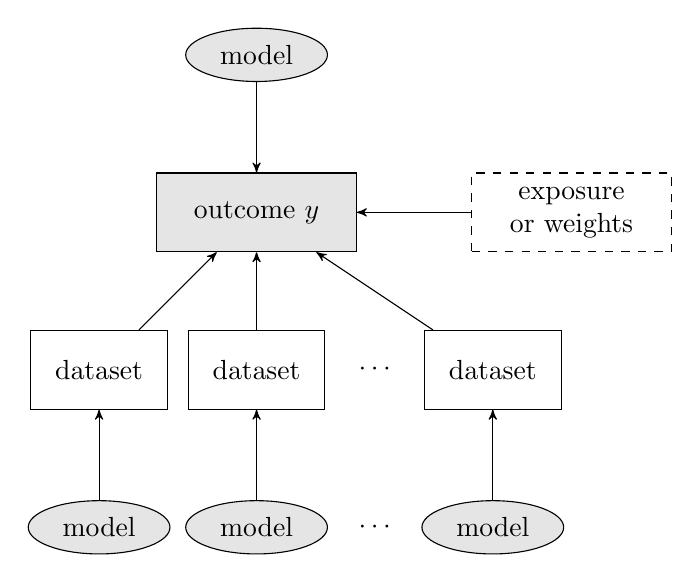
\begin{tikzpicture}
\tikzset{
   node distance = 2cm, >=stealth',
   array/.style = {rectangle, draw, minimum width = 2.3cm, minimum height = 1cm, text width = 2.3cm, align = center},
   array_obs/.style = {array},
   data/.style = {array, minimum width = 1.5cm, text width = 1.5cm},
   array_unobs/.style = {array, fill = black!10},
   model/.style = {ellipse, draw, fill = black!10, minimum width = 1.8cm} 
 }
  \node [array_unobs] (y) [] {outcome $y$};
  \node [array_obs] (ew) [right of = y, dashed, xshift = 2cm] {exposure or weights}
        edge [->] (y);

  \node[model] (model_y) [above of = y] {model}
        edge [->] (y);

  \node[data] (data_first) [below of = y, xshift = -2cm] {dataset}
        edge [->] (y);
  \node[data] (data_second) [right of = data_first] {dataset}
        edge [->] (y);
  \node[] (dots_data) [right of = data_second, xshift = -0.5cm] {$\cdots$};
  \node[data] (data_last) [right of = dots_data, xshift = -0.5cm] {dataset}
        edge [->] (y);

  \node[model] (model_first) [below of = data_first] {model}
        edge [->] (data_first);
  \node[model] (model_second) [below of = data_second] {model}
        edge [->] (data_second);
  \node[] (dots_model) [right of =model_second, xshift = -0.5cm] {$\cdots$};
  \node[model] (model_last) [below of = data_last] {model}
        edge [->] (data_last);


\end{tikzpicture}

\end{document}